\section[An introduction to the red thread for this thesis]{An introduction to the red thread for this thesis}
\label{section_read_thread} 

\epigraph{{An effective \textcolor{red}{red}} thread stop examiners from seeing `red'}{Anon (1964--on)}

A `red thread'~\footnotemark 
includes the core message of the thesis that's intended to keep the reader on track throughout the thesis. Here it's being used primarily to help me keep my work on message and enable me to discard topics and material that are too far removed from the red thread. This chapter is not written for publication, however some of the contents may be incorporated into the overall thesis.

\footnotetext{The term red thread is used in Scandinavian schools according to \href{https://writingcooperative.com/red-thread-and-other-writing-guidelines-4910b0d0d395}{‘Red Thread’ and Other Writing Guidelines}. An example of applying a red thread to a thesis is provided in \href{https://patthomson.net/2018/04/02/thesis-knowhow-how-the-contribution-can-create-coherence/}{thesis knowhow – “the contribution” can create coherence}. Tips on applying a red thread to improve a thesis are provided by a highly experienced PhD examiner in \href{https://threadreaderapp.com/thread/1192531751949737986.html}{Thread}. Others use a different colour, e.g. a \href{https://phdinahundredsteps.com/2015/05/26/spinning-the-golden-thread-that-can-sew-your-phd-together/}{a golden thread that can sew a PhD together}, and it may simply be a thread as follows: \href{https://www.thephdproofreaders.com/structure-a-phd/how-to-find-the-thread-that-runs-through-your-phd-thesis/}{How to find the thread that runs through your PhD thesis}.}

A key maxim for me is to: \emph{Always connect software engineering, mobile analytics, with the aim of improving reliability of mobile apps for end users.}



\clearpage
\section{Red Thread for the introduction chapter}~\label{red-thread-introduction}
Main chapter: \secref{chapter-introduction}.

Mobile apps are ubiquitous and used by billions. These apps, %10 words
the software tools, and their ecosystem are all imperfect therefore failures will occur and some will adversely affect the user experience and have knock-on effects. %25 words

This research uses mobile analytics to help developers of real world apps understand reliability failures, address the causes, and deploy new releases with improved reliability. %25 words
Source, value, and impact are also considered of doing so, as are real-world constraints. %15 words


\section{Red Thread for the Literature Review}
Main chapter: \secref{chapter-related-work}.


\section[Research methodology]{Research methodology}
Main chapter: \secref{chapter-methodology}. 

Empirical studies are highly appropriate and therefore used. They include complimentary primary and secondary research methods. Common threads facilitate comparisons and generalising aspects of the research. %26 words

\clearpage
\section{Red Thread for the Empirical Studies}
\label{section-empirical-studies-red-thread}

\subsection*{Notes I need to apply}
Each case study needs to be formatted consistently so that the reader can find and compare any of them with any of the others, and establish patterns and connections as they're reading them, if indeed there are intentional patterns, orderings, and so on (beyond chronological).

``Empirical research methods in software engineering"~\citep{Wohlin2003_empirical_research_methods_in_software_engineering} introduces four research methods for empirical research in software engineering: 1) controlled experiments, case studies, surveys, post-mortem analyses. Each of these has been used during the research to some extent.

A controlled experiment formed the backbone of the initial Kiwix Android app case study, then this case study applied the results of the experiment to determine whether similar improvements were achievable across the set of the project's custom Android apps. % They were...

There are a variety of in-depth case studies for specific apps within projects. These were augmented by obtaining the experiences of developers of additional Android apps who were surveyed (interviewed) on a common theme of their use and experiences with using mobile analytics services. 

After the case studies were completed, a form of post-mortem analysis identifies adverse effects of entropy returning when development teams stop paying active attention to addressing issues reported through mobile analytics.


The research combines various forms of empirical studies. These include:
\begin{itemize}
    \item Primary Research: Various \textbf{app case studies} each centered around a development team who are responsible for one or more related Android apps
    \item Secondary Research: Investigating the logging practices of developers of opensource Android apps that incorporate Google's Firebase Analytics service
    \item Primary Research: small experiments that were not appropriate in the main app case studies.
    \item Primary Research: interviews with app developers on their use of mobile analytics - indirect (secondary?) experiences of the services and tools.
    \item Primary Research: collaborations with two mobile analytics engineering teams: Google and Iteratively. 
    \item Secondary Research: Literature Review.
\end{itemize}

\subsection{Coherence throughout the case studies, in particular}


\subsection{Dimensions of the app case studies}
The following list is a proposed set of properties each case study would include:
{\small
\begin{itemize}
    \itemsep0em
    \item Role of the researcher?
    \item What are the focal points in this case study?
    \item Development practices of the project?
    \item Analytics sources: External, external + crash reporting, external + commercial internal, external, internal, and proprietary?
    \item Engagement level of the team?
    \item Privacy concerns?
    \item What opportunities did the case study present?
    \item What were the objectives (when I started the case study) compare and contrast with what actually happened? 
    \item What were the \textbf{F}indings and \textbf{I}nsights gleaned from each?
    \item What were the limitations of the tools that restricted the abilities to effect improvements? What were the limitations of the engineering practices that limited the improvements?
\end{itemize}
}

\begin{landscape} % Rotates the table into a landscape page in the generate PDF.
\definecolor{Gray}{gray}{0.9}
\begin{table}
    \setlength\extrarowheight{3pt} % provide a bit more vertical whitespace
    \captionsetup{size=footnotesize}
    \centering
    \tiny
    \tabcolsep=0.06cm
    %\rowcolors{1}{green}{pink}
    \begin{tabular}{lrrlllllllll}
        \mycolumnheading{1.9cm}{Case Study} &\mycolumnheading{0.9cm}{Apps} &\mycolumnheading{1.1cm}{Active Installs} &\mycolumnheading{1.6cm}{Role of Researcher} &\mycolumnheading{2.0cm}{Main Research Focus} &\mycolumnheading{2.0cm}{Development Practices} &\mycolumnheading{1.5cm}{Mobile Analytics} &\mycolumnheading{3.5cm}{Case Study Objectives} &\mycolumnheading{1.4cm}{Privacy} &\mycolumnheading{2.5cm}{Opportunities} &\mycolumnheading{3.2cm}{Findings} \\
        \toprule
        \rowcolor{Gray}
        Catrobat &2  &70.9K  &Coach         &Experiment &Sophisticated  &Crashlytics    &M.A. vs. Clean Code          &Strong        &Opensource          &Immediate improvements \\
                 &   &190K   &Observer      &Control     &\textit{ditto} &              &Control for above           &\textit{ditto} &\textit{ditto}      &N/A \\ 
        
        \midrule
        \rowcolor{Gray}
        C1       &1  &1M+   &Consultant     &at Scale   &Laminar        &Multiple       &Stability, Ways of Working   &Known        &Large-scale   &Rich \\
        \midrule
        GTAF     &11 &1.1M  &Observer       &Priorities &Team+          &Miscellaneous  &Accurate local language apps &Strong       &Distinct view &Their priorities \\
        \midrule
        \rowcolor{Gray}
        Kiwix    &1  &150K  &Embedded       &P-o-C      &Team+          &Android Vitals &Suppress crash rate          &V.Strong     &Open, \nth{1} case study &It works!\\
        \textit{-"-} WikiMed (EN) &1  &58.9K &Observer       &Control    &\textit{ditto} &\textit{ditto} &Control for above            &\textit{ditto} &\textit{ditto} &\textit{ditto} \\
        \rowcolor{Gray}
        \textit{-"-} Custom apps &16 &222K  &Observer       &Scaling    &\textit{ditto} &\textit{ditto} &Measure scaling              &\textit{ditto} &\textit{ditto} &\textit{ditto} \\
        \midrule         
        LocalHalo &1 &1.1K  &Observer       &Startup    &Cross-platform &Sentry.io      &New business view            &Unknown   &React-Native app &\\
        \midrule
        \rowcolor{Gray}
        Moodspace &1 &19.2K &Observer       &Startup    &1 core dev.      &Crashlytics    &New business view            &Unknown   &            &Feedback on M.A.\\
        \midrule
        Moonpig  &1  &138K  &Observer       &Firebase   &Clean Code     &Firebase       &Leading edge practices       &Known     &Firebase insights &Insightful \\ 
        \midrule
        \rowcolor{Gray}
        Big C's  &10\textsuperscript{1} &10\textsuperscript{7} &Observer &Multi-teams &N/A &N/A      &Large corporates         &Unknown   &Big picture &   \\
        \midrule
        Analytics tools &10\textsuperscript{6} &10\textsuperscript{9} &Various &Trustworthiness &Various &Various &Improve the tools &Commercial &Bleeding edge &Flaws in tools \&services \\
    \end{tabular}
    \caption{Overview of App Case Studies}
    \label{tab:overview_of_app_case_studies}
\end{table}
\end{landscape}
%%%% Notes on compressing tables
% https://tex.stackexchange.com/questions/10766/how-to-make-really-wide-tables-narrower
% https://stackoverflow.com/questions/2563498/making-latex-tables-smaller
% https://en.wikibooks.org/wiki/LaTeX/Tables#Resize_tables 
% Smaller text finally worked after applying the tips from https://tex.stackexchange.com/a/56011/88466
% Row colors https://texblog.org/2011/04/19/highlight-table-rowscolumns-with-color/
% Rotate table https://tex.stackexchange.com/questions/370393/how-to-rotate-the-large-table-and-caption/370394
% Add a footnote https://tex.stackexchange.com/a/66641/88466
% Improvements in the formatting of the generated table https://tex.stackexchange.com/a/327977/88466

\begin{comment}
MUST-DO
The monster table needs a column for what each study contributes to my thesis.
Any other pertinent information to add ?
What viewpoints did each case study provide?
Merge Research Focii and case study objectives vs. the objectives of the case study team.
The long view is useful to highlight of various case studies. Repeated and long-term engagement and access to analytics and/or code.
Mini-table for each case study, include the active study period, follow over ...
The role of the case study.
\end{comment}

\newthought{Joe's suggestions}
\textit{Note: these will be merged into the rest of the thesis, here as a reminder until that's done.}

Joe is an industrial colleague. He proposed each case study could be formatted as a mini-paper with an abstract per case study.
{\small
\begin{itemize}
    \itemsep0em
    \item Which of the research questions does it answer?
    \item What’s the context? Mobile app? Web? Reporting tools? Library?
    \item What’s the company? Org structure? Communication tools?
    \item What tools were used? MS App Center, Android Vitals, etc. Crashlytics, Testing Frameworks, Collaboration tools,
    \item Team structure?
    \item How many users?
    \item Do the devs have access to the tools? how integrated into the development practices?
    \item Future work for each case study.
\end{itemize}
}
There are some overlaps and similar topics between the suggested dimensions of each case study and Joe's proposed list. TODO These two lists need to be harmonised, non-essential topics may be pruned from the combined list.


\subsubsection{Revised set of Marian's comments from our call on \nth{1} Sept 2021}

\newthought{The map is vital.}

There new tables aim to provide a partial map for the examiners so they don't get lost or side-tracked. They also help to clarify the thinking and make the case studies more consistent and coherent.

\begin{enumerate}
    \item \ref{tab:empirical-studies-research-perspective} \nameref{tab:empirical-studies-research-perspective}
    \item \ref{tab:empirical-studies-their-characteristics} \nameref{tab:empirical-studies-their-characteristics}
    \item \ref{tab:empirical-studies-findings-and-results} \nameref{tab:empirical-studies-findings-and-results}
\end{enumerate}

Notes: The previous table \ref{tab:overview_of_app_case_studies} \nameref{tab:overview_of_app_case_studies} may eventually be retired and removed from this red-thread. Another table, on the analytics tools, is also worth me creating.

Ideally a drawn map would complement these tables.


\newthought{Demonstrate competence as a researcher}
You need to be more precise in how you report the methodology, e.g., the case studies actually use mixed methods (not just the expansion). A methodology combines reasoning with the method. You need to convey rigour within the constraints of access to case studies.

At some point, you need a 'map' of the case studies:  these need to include the: case, methods, purpose...  This should give the reader an overview of what each contributes and where they overlap.


\newthought{Explain the challenges of anyone being permitted by teams to access their sensitive data, the opportunistic access and rigour applied in the case studies.}

Maximise my ability to make systematic use of what was pragmatically available: Opportunistic access, then I worked systematically and rigorously. Demonstrating the demands of rigour is vital. Explicit reporting of what I had and the efforts I made to handle the data systematically and be vigilant for bias. This helps avoid the case studies being considered as anecdotal. Amplify with the dialogues I had as part of the teams.

Start with what data did I collect and how I collected it. The case studies with similar sources of data can be compared which multiply the contribution.

Aim to explain what are the issues that arose in each case study?
A clear rationale needs to be provided. 

It's wise for the thesis to demonstrate there's a really clear audit trail and justification for the conclusions.

\begin{itemize}
    \item Characterise the empirical studies.
    \item Make explicit what data was collected and for what purpose. 
    \item Separate insights into a separate table. 
\end{itemize}

Quality of reporting of the empirical work is key

\newthought{Be Orthogonal and separate concerns}

MUST-DO Separate the reporting from the discussion.


\begin{landscape} % Rotates the table into a landscape page in the generate PDF
\begin{table}
    \centering
    \tabcolsep=0.06cm
    \tiny
    \begin{tabular}{lllll}\toprule
    Case Study                 & Role of Researcher &  Primary Research Method   & Research Opportunities             & Research Purpose \\
    \midrule
    Kiwix                      & Embedded           & Quasi-experiment   &The proof-of-concept      & The experiment \\ 
     \textit{-"-} WikiMed (EN) & Observer           &                    &Control for the above app & The control  \\
    \textit{-"-} Custom apps   & Observer           &                    & Evaluate scalability     & \textit{pico} generalisation \\
    \midrule
    Catrobat                   & Coach              & Quasi-experiment   &                          & Compare Mobile Analytics with Clean Code \\
     \textit{-"-}              & Observer           &                    & Establish baseline       & The control  \\
     \midrule
    C1                         & Consultant         & Hybrid/Mixed & Large scale complex commercial & Mission-critical view \\
    GTAF                       & Interviewer        & Semi-structured interview & Add'l perspective & Exploring the long tail \\
    LocalHalo                  & Interviewer        & Semi-structured interview & Add'l technologies & Hybrid Programming and tools \\
    Moodspace                  & Interviewer        & Semi-structured interview & Small startup &Bootstrap view \\
    Moonpig                    & Interviewer        & Semi-structured interview & Leading edge view & Mature, innovative, vanguard dev. practices \\
    Analytics tool providers   & Various            & & `Behind the curtain' & Learn about the providers' perspectives \\
    \bottomrule
    \end{tabular}
    \caption{Empirical Studies: the research perspective}
    \label{tab:empirical-studies-research-perspective}
\end{table}
\end{landscape}


\begin{table}
    \centering
    \tabcolsep=0.06cm
    \footnotesize
    \begin{tabular}{lcrcll}\toprule
    Case Study               & Apps                 & Reach & Project context & Mobile Analytics Tools\textsuperscript{*}  &Dev. practices  \\
    \midrule
    Kiwix                    &                    1 &  150K & Wikipedia, FOSS            & GPC with AV &          Team+ \\ 
     \textit{-"-}            &                    1 & 58.9K & \textit{-"-}   & GPC with AV & \textit{ditto} \\
     \textit{-"-}            &                   16 &  222K & \textit{-"-}   & GPC with AV & \textit{ditto} \\
    Catrobat                 &                    1 & 70.9K & Coding, FOSS            & Crashlytics &  Sophisticated \\
     \textit{-"-}            &                    1 &  190K & \textit{-"-}   & GPC with AV & \textit{ditto} \\
    C1                       &                    1 &  1M+  & Mission-critical &    Multiple &        Laminar \\
    GTAF                     &                   11 &  1.1M & Another app category             &Miscellaneous &          Team+ \\
    LocalHalo                &                    1 &  1.1K & Risky early startup &   Sentry.io & Cross-platform \\
    Moodspace                &                    1 & 19.2K & Medical    & Crashlytics &        Startup \\
    Moonpig                  &                    1 & 138K  & E-commerce &    Firebase &     Clean Code \\
    Analytics tool providers &10\textsuperscript{6} &10\textsuperscript{9} & No &  Several &        Various \\
    \bottomrule
    \end{tabular}
    \caption[Case Studies: their characteristics]{Case Studies: their characteristics \\ {\tiny * All the apps used GPC with AV; one of the tool providers \emph{is} GPC with AV \\ FOSS = Free and Open Source Software}}
    \label{tab:empirical-studies-their-characteristics}
\end{table}

To consider: project context, the drivers for the project, and what's noteworthy about the case study to help the reader?

Each of the in-dept case studies had their own objectives from participating in the research, and a common need from their perspective was to try and reduce the reported crash rate for at least one of their Android apps.

\begin{landscape} % Rotates the table into a landscape page in the generate PDF
\begin{table}
    \centering
    \tabcolsep=0.06cm
    \tiny
    \begin{tabular}{lllll}\toprule
    Case Study                  &Evidence    &Results               &Main Findings             &Insights  \\
    \midrule
    Kiwix                       &Code and Analytics results &3x improvement        &Targeted bug fixes v.effective &Visibility drove action \\ 
     \textit{-"-}               &Baseline         &stable                &                     & \\
     \textit{-"-}               &Code and Concrete results &reduced crash-rates   &The approach scaled  &Lead dev. took ownership \\
     \midrule
    Catrobat                    &Corroboration, crashlytics &2x improvement     &Immediate improvements &Ongoing ownership is vital \\
     \textit{-"-}               &Baseline         &stable                &                     & \\
     \midrule
    C1                          &Concrete results &Multi-faceted improvements &OKRs achieved & Rich, multi-faceted \\
    GTAF                        &Corroboration    &                      &Historical perspective &Their priorities  \\
    LocalHalo                   &Add'l M.A. tool  &                      &Sentry.io &Limitations of GPC with AV for hybrid apps \\
    Moodspace                   &Corroboration    &                      &Effectiveness of good app design &Feedback on M.A. \\
    Moonpig                     &Corroboration    &                      &Effectiveness of engaged, motovated teams &Insightful \\
    Analytics tool providers    &Their priorities &Improvements made to their tools & Flaws in tools \& services &This research is v.valuable \\
    \bottomrule
    \end{tabular}
    \caption{Case Studies: findings and results}
    \label{tab:empirical-studies-findings-and-results}
\end{table}
\end{landscape}

\begin{comment}
MUST-DO
Disambiguate Contributions into Evidence, Insights, and the Distinct Opportunity/Perspectives it provided. Impact on the teams.
Consider an Insights table, mapping back on to the case studies. 
Insights in practices of the development teams. 
Try creating an evidence table. 
\end{comment}

\subsection{Classifications of Mobile Analytics tools}
The case studies also facilitated the study of various mobile analytics tools. A map of these tools and the case studies they were used in may help the reader (and the author). Here are suggested topics to consider for each of these tools.
\begin{itemize}
    \itemsep0em
    \item To consider: which projects was the tool used in/relevant to?
    \item What was the tool used for?
    \item What insights did we glean from using the tool?
    \item If anythings made the tool distinctive, what were those things and why are they distinctive in the context of developers using mobile analytics?
\end{itemize}

\subsection{Contributions of the empirical studies to the research question}
For ease of reference, the main research question is:
\begin{quote}
    \emph{How can applying analytics improve software development and software testing for mobile apps in practice?}    
\end{quote}
Sub-questions focus on sources, value and impact. 
\begin{landscape} % Rotates the table into a landscape page in the generate PDF
\begin{table}
    \centering
    \tabcolsep=0.06cm
    \tiny
    \begin{tabular}{lllll}\toprule
    Case Study                  &Results                &Sources                &Value             &Impact within the case study  \\
    \midrule
    Kiwix                       &3x improvement         &GPC with AV            &Crash rates improved &  \\ 
     \textit{-"-}               &stable                 &GPC with AV            &Crash rates improved &  \\
     \textit{-"-}               &Reduced crash-rates    &GPC with AV            &Crash rates improved & Dev. lead took ownership. \\
     \midrule
    Catrobat                    &2x improvement         &GPC with AV, Fabric Crashlytics &Crash rates improved &Led to dev team visiting Poland. \\
     \textit{-"-}               &stable                &   &                  & \\
     \midrule
    C1                          &Multi-faceted improvements &In-house, Google Analytics, App Center &OKRs achieved &Sporadic \\
    GTAF                        &                      &TBC &High crash rates addressed &Pareto-like application \\
    LocalHalo                   &                      &sentry.io &Critical failures are fixed & \\
    Moodspace                   &                      & & & \\
    Moonpig                     &                      &Firebase & & \\
    Analytics tool providers    &Improvements made to their tools &GPC with AV, iterative.ly  &This research is v.valuable &Demonstrated by results \\
    \bottomrule
    \end{tabular}
    \caption{Empirical Studies: contributions to research questions}
    \label{tab:empirical-studies-contributions-to-research-questions}
\end{table}
\end{landscape}
%\href{section-empirical-studies-red-thread}{\nameref{section-empirical-studies-red-thread}} includes a table of the role the researcher played in each case study together with other pertinent details.

\subsection{Observations on the case studies}
The research includes several aspects seldom studied owing to the challenges of obtaining the case studies, for instance from behind the curtain in commercial projects with over a million users, and from sources again seldom visible to researchers \emph{i.e.} of mobile analytics for real-world mobile apps.



\clearpage
\section[Phases of a release]{Phases of a release\\ \small{(Possibly integrate into Introduction, or into Preparing the Ground (Ch3))}}

%%% Thanks to
% https://tex.stackexchange.com/questions/69550/how-can-i-add-a-subtitle-to-a-section-title
% If I want to get fancy then https://tex.stackexchange.com/questions/417429/how-to-make-subheadings 

\begin{figure}
    \centering
    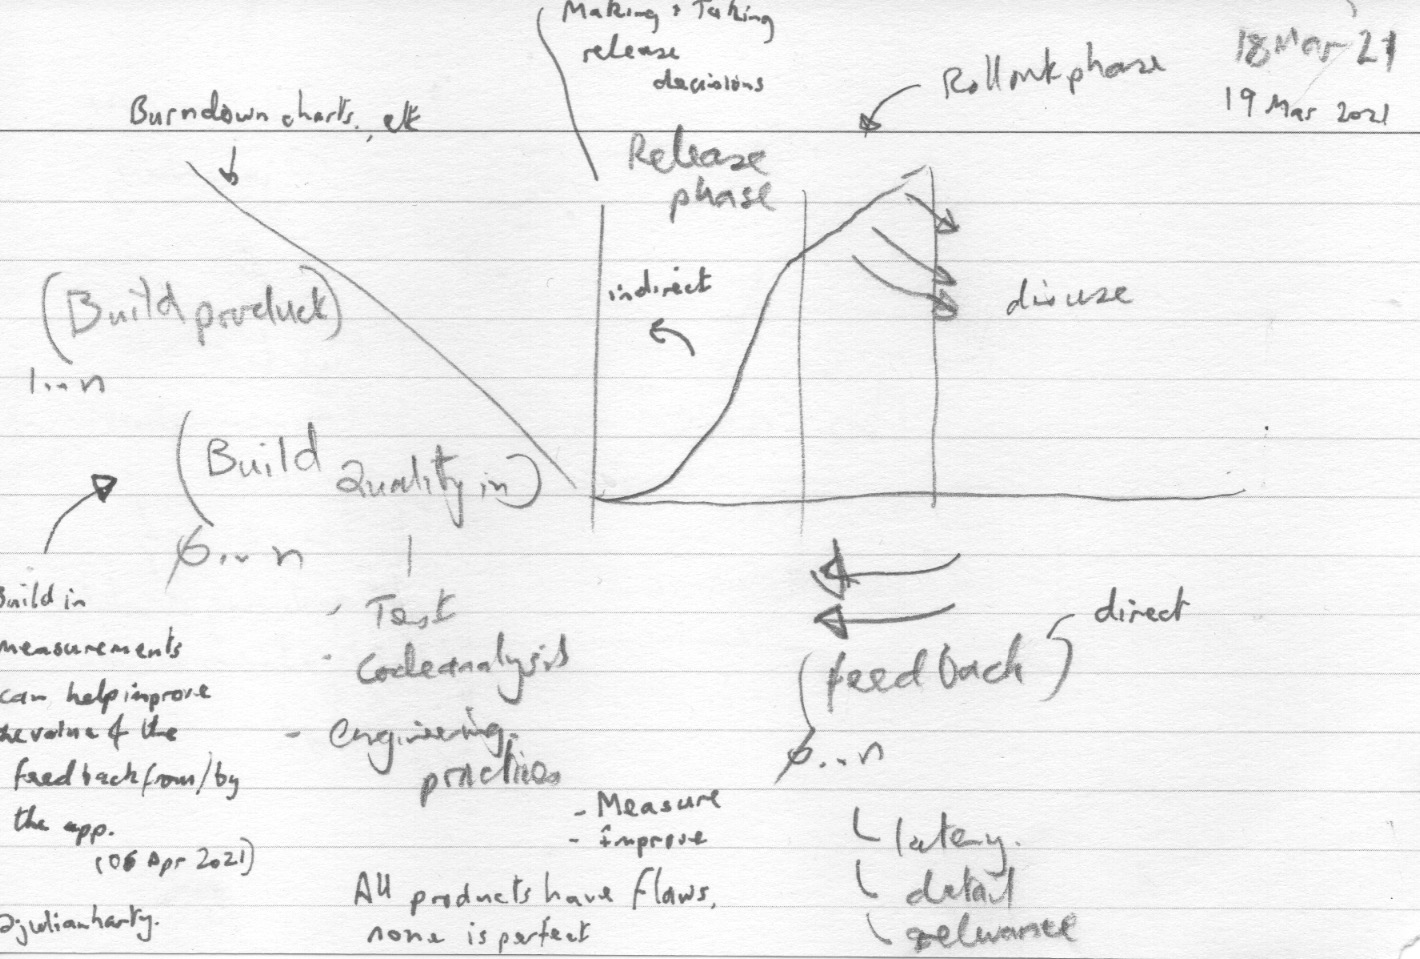
\includegraphics[width=15cm]{images/rough-sketches/Red-Thread-Rough-Sketch.jpeg}
    \caption{The lifecycle of a release and where mobile analytics provides feedback}
    \label{fig:red-thread-for-this-thesis}
\end{figure}

For any given release of a mobile app there are at least three material phases in order for the release to be used:
\begin{enumerate}
    \item Building the product: which may incorporate practices and tools intended to ship a `quality product'. Some teams also incorporate logging and reporting to help measure the behaviours of the app in use, post release.
    \item The Release: For some projects this may be as simple as uploading a new binary and making it fully available. For others they may incorporate decisions and mechanisms to make each release with the aim of de-risking any undesirable/adverse effects of the new release.
    \item Deployment: Deployment occurs when end users install and start using the release of the app. Both the app store and the end users affect when this occurs. App developers can try to hasten when users install the latest release through various mechanisms, for instance through implementing and mandating users upgrade their current release.
\end{enumerate}

Figure~\ref{fig:red-thread-for-this-thesis} illustrates these three phases together with some of the dynamics \emph{e.g.} of rollout and disuse of a release, and of feedback from whatever sources that the development teams can choose to pay attention to and apply. These phases are part of a longer lifespan of the release that includes an often long-term postdelivery period~\citep[pp 156-157]{evans2004_achieving_software_quality_through_teamwork} where users use the release until it is decommissioned or replaced with a subsequent release.

\begin{figure}
    \centering
    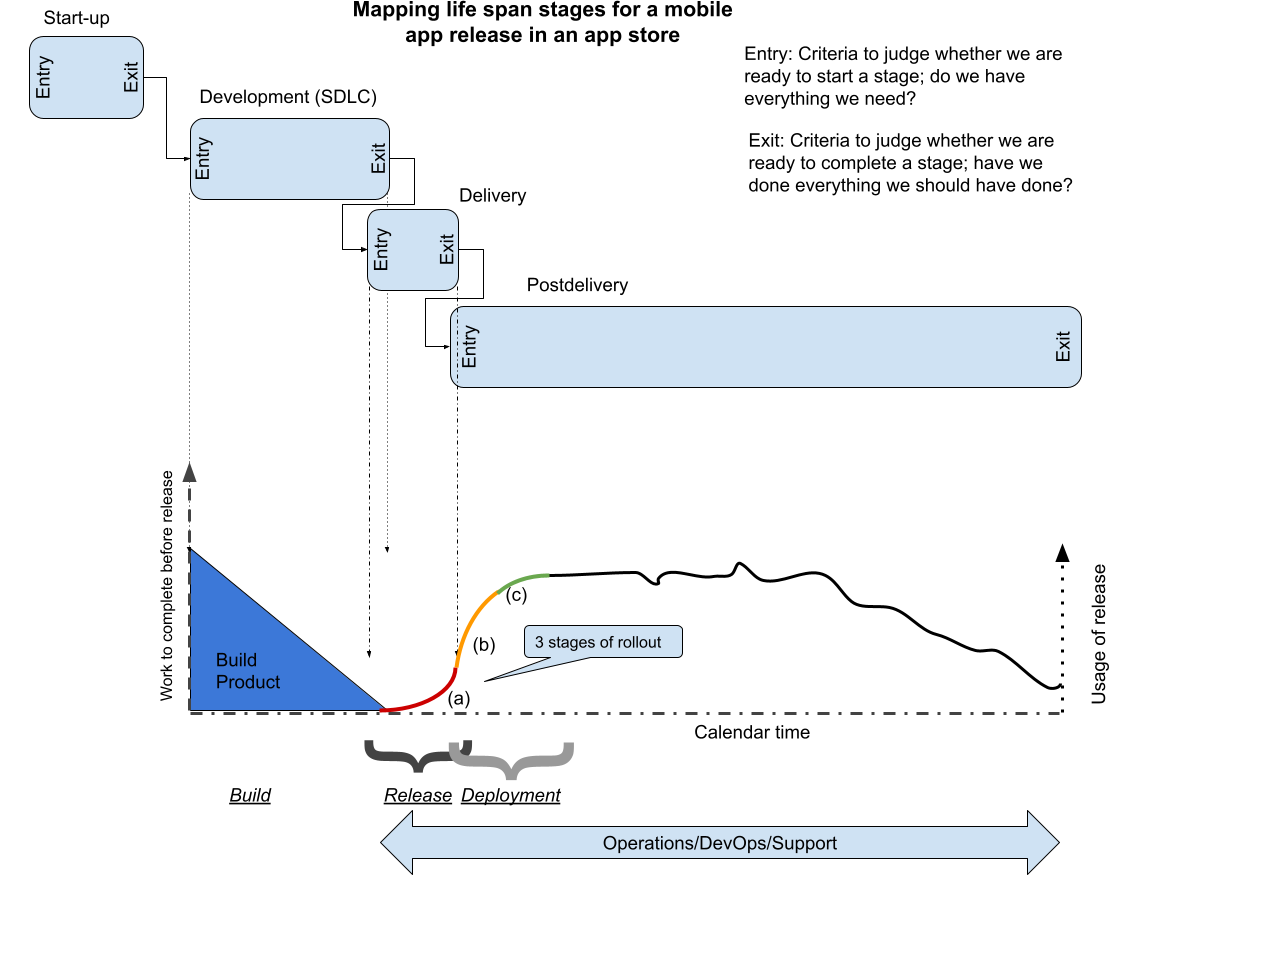
\includegraphics[width=16cm]{images/my/mobile-app-life-span-stages.png}
    \caption{Mapping life span stages for a mobile app release in an app store}
    \label{fig:mobile-app-life-span-stages}
\end{figure}

Figure~\ref{fig:mobile-app-life-span-stages}~\footnote{Source of figure, Google Drive file: \href{https://docs.google.com/document/d/1d4B5l1tlpclHdKwY8W00qchiCV2YK5JjJP8TbkRHcjQ/edit}{Mobile app life span stages}.} compares a revised version of the `Life span stages' Figure in~\citep[p.155]{evans2004_achieving_software_quality_through_teamwork} mapped approximately to the three stages first illustrated in Figure~\ref{fig:red-thread-for-this-thesis}. Mobile app releases in an app store extend the Delivery which may also overlap either or both the development and the postdelivery life span stages. The overlap with the development stage is because the development is not complete until the app store accepts/approves the release (this may include pre-launch checks, automated testing, and so on depending on the app store). The overlap with deployment happens as releases are often released incrementally initially to a small percentage of the userbase - at least some of the users in that percentage will install the new release, until the percentage has been achieved. Meanwhile at least some of those users will use the app which will then mean the release is operational and may need operational support.


This research found that developers are able to materially improve the stability/reliability~\footnote{For Android Google used the term `stability' when they describe their Android Vitals service which is incorporated into Google Play Console. It effectively measures reliability for two specific types of failure: crashes and ANRs. An overview of Android Vitals is available online from various Google and Android sources including~\citep{android_vitals_overview_2019, android_vitals_best_practices}. HP also used the term `~\href{glossary-stability}{stability}' to measure crashes in mobile apps.}
%
of their mobile apps when they use the results of mobile analytics to assess the stability/reliability, identify groups of failures, triage the failures, and address the ones they decide to action. Where project teams stop paying attention to this process the failure rate increases of their new releases - the apps tend to entropy and failure.

Diligent developers and development teams can materially improve the stability/reliability of their apps through applying good coding, design and architecture patterns. Even these practices do not guarantee the releases will always be trouble-free. By paying ongoing attention to analytics during development, testing, and the rollout of releases flaws can be identified before the release reaches the majority of the userbase and teams can ameliorate the effects of many of the flaws.
\clearpage 


\subsection{When can identified issues be addressed?}
To address issues they need to be identified and a practical improvement determined. The practical improvement may be an outright fix, or a workaround, or an amelioration, etc. The questions for the development team include where and when the improvements can be applied to improve the reliability for the end users of their app.

Some issues can be ameliorated externally to the app, for instance though changes to servers that support API requests from apps, however many need changes to the app in order to be effective.

For apps released as compiled binary files (the vast majority in iOS and Android app stores), improvements are generally made to a subsequent release than the one(s) where the failures have been occurring\footnotemark. And these subsequent releases need to be installed by the user population and used similarly in order to determine whether the improvements were worthwhile. Some users keep older releases and others stop using the app so 100\% rollouts of subsequent releases are not practical. (For apps that only ever had one release then 100\% rollout is \emph{de-facto}.)

\footnotetext{
  There are various ways that a binary \emph{can} be patched or updated \textit{in-situ}. Indeed various security attacks are performed using this approach, as, for instance,~\citep{poeplau2014_execute_this_unsafe_android} discussed. Around April 2013 Google changed their policy for Google Play to forbid Android apps from modifying, replacing or updating it's own APK binary code outside Google Play's update mechanism (the policy is still available on the Internet Archive Wayback Machine~\href{https://web.archive.org/web/20130426113437/https://play.google.com/about/developer-content-policy.html}{Google Play Developer Program Policies}). In 2019, Google provided developers with an API that developers can embed into their Android app in order to prompt users to update the app using Google Play~\citep{android_in_app_updates}. 
}




\newthought{Record and replay/playback}
Recreate the `journey' (however relevant context may be missing or different and therefore affect the results and conclusions). Various reasons why recreating the journey is desirable e.g. to reproduce failures to help understand their characteristics and causes, to learn indirectly by observing and visualising the journey. \emph{c.f.} heatmapping. Record and replay offers the possibility of moving beyond using breadcrumbs as it is intended to record sufficient information to reproduce the use of an app. However there are various limitations in the tooling, the techniques, and at least as importantly the unacceptability of recording end user sessions on their devices using production releases of apps downloaded from the app store. 

\newthought{Prior art in record and replay/playback}
\textit{FYI This will be moved to the Related Work chapter}
TBC


\clearpage
\section[Practical aspects of using analytics]{Practical aspects of using analytics \\ \small{(Possibly migrate to the Conclusion? else the Discussion?)}}
Analytics providers have a major influence on the efficacy of the application of mobile analytics. There are limitations and flaws in the various tools this research has encountered regardless of their source (\emph{e.g.} in-house proprietary, opensource, free and paid-for commercial proprietary offerings). Nonetheless, flawed offerings are still able to be used to deliver improvements in the mobile apps. Specialised startups such as Iteratively aim to increase the coherence of embedded analytics (those embedded into the apps) while also increasing compliance. HP's AppPulse Mobile provided no-code analytics for mobile apps where their tools automatically instrumented the binary to add the analytics; several providers offered GUI interaction recording and `heatmaps' generated using aggregated recordings of touch screen interactions.

Those who applied the results of mobile analytics were able to increase the stability/reliability of their mobile apps. The amounts of improvements varied based on various factors such as:
\begin{itemize}
    \itemsep0em
    \item The starting point for the app.
    \item The amount of ongoing engagement of the development team.
    \item The choices of mobile analytics services and the use of proactive event recording using the related analytics libraries.
    \item The sources and causes of some of the issues being reported - some where far harder to diagnose than others, and several originated outside the actually codebase of the mobile app where it might be impractical to truly fix the source of the issue.
\end{itemize}

\noindent
\rule{\textwidth}{0.4pt}

\clearpage
\section{Where's my current focus?}
It's in several areas:
\begin{itemize}
    \item Create a presentation to sum up the research.
    \item Provide coherence and consistency to the empirical studies. Learn about methodologies applied to empirical studies.
    \item (Ongoing) Some additional development of the possible framework in Section 0.6 and Figure 0.3
    \item (Ongoing) On the related work chapter, adding various references and starting to develop these into coherent discussions of these works, the gaps in research, etc.
    \item (Done) To revise the red-thread for the case studies and create three distinct tables as per my discussion with Marian and then flesh out and organise the case studies.
\end{itemize}

